\scanpage{148}
\mspage{1}
% archive foliation: 147
Additif Esquisse d'un Programme.

\uline{Voisinages tubulaires} d'\uline{une partie}
\inserted{\unsure{modéré|modérée}} \uline{quelconque} d'un
espace modéré (\unsure{resp.} $A$). \unsure{PS|A} réduit à
un point.

\deleted{\unsure{comme} ``bord''}

I) Sous-espace modéré ``bordant'' \deleted{\illegible{1}} $B$ d'un espace
modéré $X$. Collier autour de $B$

(\deleted{$B\times I\unsure{\longrightarrow}$} $B\subset C\subset X$,
$C$ vois. de $B$, $\exists\ C\xleftarrow[\sim]{\varphi}B\times I$,
\inserted{et $\dot C=\varphi(B\times\{1\})$}.

avec \deleted{$B\unsure{\simeq}B$}
\diagram{\begin{tikzcd}[column sep=small]
& B \arrow[dl] \arrow[dr,"b\mapsto(b,0)"] & \\
C \arrow[rr,"\sim"] && B\times I
\end{tikzcd}}
\margin{Collier \deleted{\illegible{1}} \inserted{strict}}
\[
I=[0,1]
\]

\margin{se donner \deleted{\unsure{aussi} $\unsure{\dot C\simeq B}$}
\unsure{aussi} $\dot C=$}
\figure{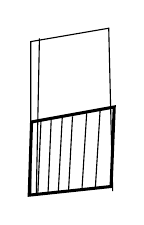
\begin{tikzpicture}[x=1cm,y=1cm]
\draw[thin] (0.02,0) -- (0.02,1.95) -- (1.01,2.12) -- (1.06,0.05);
\draw[thin] (0.09,0) -- (0.13,1.99);
\draw[line width=1.1pt] (0,0) -- (0.03,0.93) -- (1.08,1.12) -- (1.04,0.11) -- cycle;
\draw[thin] (0.11,0.03) -- (0.15,0.95);
\draw[thin] (0.24,0.04) -- (0.28,0.97);
\draw[thin] (0.37,0.05) -- (0.42,0.99);
\draw[thin] (0.50,0.06) -- (0.55,1.00);
\draw[thin] (0.67,0.07) -- (0.73,1.04);
\draw[thin] (0.84,0.09) -- (0.90,1.07);
\end{tikzpicture}}

\deleted{($(B,1)$ est bordant dans}

($\dot C$ est bordant dans \deleted{$B$} $(C\setminus\dot C)$)
Collier rigidifié

\uline{Conj} $\unsure{\Rightarrow|\to}$ Soit $B$ bordant dans $X$

a) $\exists$ Collier $(C,\dot C)$ donc aussi collier strict

b) ``L'espace'' des colliers stricts est contractile.

c) L'espace des \deleted{colliers \inserted{rigidifiés} et \unsure{stricts}}
\deleted{est fibré sur}
colliers \deleted{\unsure{stricts}} est contractile, ou en-
core : l'espace des autom. d'un
collier, induisant l'identité de $B$
(et ``libres'' sur $\dot C$) est contractile.

i.e. le choix d'un collier\inserted{strict}, ou d'un collier \inserted{strict} rigidifié,
ou d'une rigidification d'un collier, est
anodin.
